% Chapter 2

\chapter{On general cosystoles and Cheeger constants}

\label{Chapter2}

When we want to determine whether a cochain is a cosystole or not or to determine the cosystolic norm of a cochain by now we only have the original definition of cosystolicity, which does not seem to be very handy. In this chapter we want to develop tools to get hands on this problem, especially by estimating the cosystolic norm in various situations and investigating the structure, how cosystoles in certain simplicial complexes are arranged.

\section{Hitting numbers and the cycle detection theorem}

In this section we want to study the (by now) most promising approach to get hands on the cosystolic norm by applying the well studied concept of hitting sets. The following definition is adopted from \cite{6} (Definition 2.1). Note, that in the referenced paper Kozlov and Meshulam used the denotation "piercing set" and "piercing number" instead of hitting set and hitting number, which both refer to the same concepts.

\begin{defi}
Let \(V\) be some set and \(\mathcal{F}\subseteq 2^V\) a family of subsets of \(V\). A subset \(P\subseteq V\) is called a \textbf{hitting set} of \(\mathcal{F}\) if we have \(P\cap F\neq\emptyset\) for all \(F\in\mathcal{F}\). The minimal cardinality which a hitting set of \(\mathcal{F}\) can attain is called the \textbf{hitting number} of \(\mathcal{F}\), denoted by \(\tau(\mathcal{F})\). For \(v\in V\) and \(F\in\mathcal{F}\) we say that \(F\) \textbf{is hit by} \(v\), if \(v\in F\).
\end{defi}

\begin{expl}\label{example1}
Let \(V\coloneqq \left\{1,2,3,4,5\right\}\) and \(\mathcal{F}\coloneqq \left\{\{1,2\}\{2,3,4\},\{1,5\},\{2,4,5\}\right\}\), then we have \(\tau(\mathcal{F})=2\), since for example \(P\coloneqq \left\{2,5\right\}\) is a minimal hitting set of \(\mathcal{F}\).
\end{expl}

Later we will talk about hitting numbers and hitting sets of families of \(k\)-chains, which we define as follows:

\begin{defi}
Let \(X\) be a simplicial complex and \(\mathcal{F}\subseteq C_k(X)\) a family of \(k\)-chains. The \textbf{hitting sets} and the \textbf{hitting number} of \(\mathcal{F}\) are defined as the hitting sets and the hitting number of the family \(\left\{\supp(F):F\in\mathcal{F}\right\}\).
\end{defi}

In \cite{6} (Theorem 2.2) Kozlov stated the following useful method to bound the cosystolic norm of a cochain.

\begin{thm}[The cycle detection theorem]\label{theorem9}
Let \(X\) be a simplicial complex, \(k\geq 1\), and \(\varphi\in C^k(X)\). Let now \(\mathcal{F}=\left\{\alpha_1,\ldots,\alpha_t\right\}\) be a family of \(k\)-cycles in \(C_k(X)\), such that \(\left\langle\varphi,\alpha_i\right\rangle=1\) for all \(1\leq i\leq t\), then we have:
\[
\|\varphi\|_{csy}\geq\tau(\mathcal{F})
\]
\begin{proof}
Let \(\psi\in C^{k-1}(X)\), then for any \(1\leq i\leq t\) we have:
\begin{align}
\langle\varphi+\delta^{k-1}(\psi),\alpha_i\rangle&=\langle\varphi,\alpha_i\rangle+\langle\delta^{k-1}(\psi),\alpha_i\rangle\notag\\
&=\langle\varphi,\alpha_i\rangle+\langle\psi,\partial_{k-1}(\alpha_i)\rangle\notag\\
&=\langle\varphi,\alpha_i\rangle+\langle\psi,0\rangle\notag\\
&=\langle\varphi,\alpha_i\rangle=1\notag
\end{align}
This means that we have \(\supp(\varphi+\delta^{k-1}(\psi))\cap \supp(\alpha_i)\neq\emptyset\) for all \(1\leq i\leq t\), so \(\supp(\varphi+\delta^{k-1}(\psi))\) is a hitting set of \(\mathcal{F}\) and we get:
\[
\|\varphi+\delta^{k-1}(\psi)\|=|\supp(\varphi+\delta^{k-1}(\psi))|\geq\tau(\mathcal{F})
\]
Since \(\psi\) was chosen arbitrarily we are done.
\end{proof}
\end{thm}

The following corollary (a special case of the preceding theorem) was also stated by Kozlov in \cite{6} (Corollary 2.3).

\begin{cor}\label{corollary1}
Let \(X\) be a simplicial complex and \(\varphi\in C^k(X)\).\\
Let now \(\mathcal{F}=\{\alpha_1,\ldots,\alpha_{\|\varphi\|}\}\) be a family of \(k\)-cycles in \(C_k(X)\), such that \(\left\langle\varphi,\alpha_i\right\rangle=1\) for all \(1\leq i\leq\|\varphi\|\) and \(\supp(\alpha_i)\cap \supp(\alpha_j)=\emptyset\) for all \(i\neq j\), then \(\varphi\) is a cosystole.
\begin{proof}
Since the supports of the cycles \(\alpha_1,\ldots,\alpha_{\|\varphi\|}\) are pairwise disjoint, we obviously have \(\tau(\mathcal{F})=\|\varphi\|\) and using the cycle detection theorem we are done.
\end{proof}
\end{cor}

\begin{expl}\label{example1a}
Consider the cochain
\[
\varphi=\left(\{1,2,4\}+\{2,4,6\}+\{2,5,6\}+\{3,4,6\}\right)^*\in C^2(\Delta^{[6]})
\]
(Figure \ref{figure1:Figure 1} illustrates how the support of this cochain can be imagined) and the family of cycles
\begin{align*}
\mathcal{F}=\{&\{1,2,3\}+\{1,2,4\}+\{1,4,3\}+\{2,4,3\},\\
&\{1,2,5\}+\{1,2,6\}+\{1,5,6\}+\{2,5,6\},\\
&\{3,4,5\}+\{3,4,6\}+\{3,5,6\}+\{4,5,6\},\\
&\{1,3,5\}+\{1,3,6\}+\{1,4,5\}+\{1,4,6\}+\\
&\{2,3,5\}+\{2,3,6\}+\{2,4,5\}+\{2,4,6\}\}\subset C_2(\Delta^{[6]})
\end{align*}
It is easy to check that we have \(\left\langle\varphi,\alpha\right\rangle=1\) for all \(\alpha\in\mathcal{F}\) and \(\tau(\mathcal{F})=4\), so we get \(\|\varphi\|_{csy}\geq 4\) by the cycle detection theorem. We can immediately see, that \(\varphi\) is a cosystole, either by the fact that we always have \(\|\varphi\|_{csy}\leq \|\varphi\|\), so in our case we have \(\|\varphi\|=4=\|\varphi\|_{csy}\), or by using the preceding corollary, since the supports of the cycles in \(\mathcal{F}\) are pairwise disjoint.\\
Note, that \(\varphi\) is even a Cheeger cosystole, since we have \(\|\varphi\|_{exp}=\frac{6}{4}\), so we know that for the example \(n=6\) and \(k=2\) the lower bound of the estimate \ref{equation1} is archieved, even though \(k+2\) does not divide \(n\).
\end{expl}

\begin{figure}[ht]
\centering
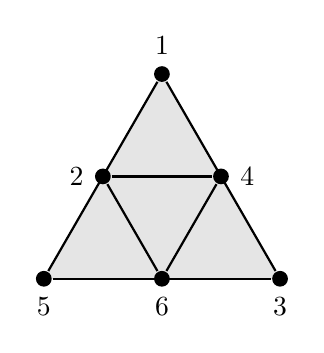
\begin{tikzpicture}[
       thick,
       acteur/.style={
         circle,
         fill=black,
         thick,
         inner sep=2pt,
         minimum size=0.2cm
       }
     ] 

	   \fill[fill=gray!20] (0,0)--(3,0)--(1.5,2.6);

       \node (a1) at (0,0) [acteur,label=below:5]{};
       \node (a2) at (3,0)[acteur,label=below:3]{}; 
       \node (a3) at (1.5,2.6) [acteur,label=above:1]{}; 
       \node (a4) at (0.75,1.3) [acteur,label=left:2]{}; 
       \node (a5) at (2.25,1.3) [acteur,label=right:4]{}; 
       \node (a6) at (1.5,0) [acteur,label=below:6]{};
  
       \draw (a1) -- (a2); 
       \draw (a2) -- (a3); 
       \draw (a1) -- (a3);
       
       \draw (a4) -- (a5);
       \draw (a5) -- (a6);
       \draw (a4) -- (a6);

\end{tikzpicture}
  \caption{The support of a $2$-Cheeger cosystole (The gray triangles represent the four $2$-simplices)}
  \label{figure1:Figure 1}
\end{figure}


To get the best possible results using the cycle detection theorem, the challenge is now for a certain cochain \(\varphi\) to find families of cycles, such that they have a large hitting number and \(\varphi\) evaluates to \(1\) on every cycle. The following construction seems to be suited well to get hands on this problem.\\
For a simplicial complex \(X\) and a cochain \(\varphi\in C^k(X)\) we define the following set of cycles:
\[
\mathcal{T}_{\varphi}\coloneqq \left\{\partial_k(\sigma):\sigma\in \supp(\delta^k(\varphi))\right\}
\]

\begin{prop}\label{proposition1a}
Let \(X\) be a simplicial complex and \(\varphi\in C^k(X)\), then we have:
\[
\|\varphi\|_{csy}\geq\tau(\mathcal{T}_{\varphi})
\]
\begin{proof}
By the definition of the coboundary map, we obviously have\\
\(\left\langle\varphi,\partial_k(\sigma)\right\rangle=1\) for all \(\partial_k(\sigma)\in\mathcal{T}_{\varphi}\) and so by the cycle detection theorem we are done.
\end{proof}
\end{prop}

Note, that in many cases even the equality \(\|\varphi\|_{csy}=\tau(\mathcal{T}_{\varphi})\) can be reached, but unfortunately this is not always true as the following example shows.

\begin{expl}\label{example1b}
Let \(\varphi\in C^2(\Delta^{[6]})\) be the cosystole from Example \ref{example1a}. We have:
\begin{align*}
\mathcal{T}_{\varphi}=\{&\{1,2,3\}+\{1,2,4\}+\{1,3,4\}+\{2,3,4\},\\
&\{1,2,4\}+\{1,2,5\}+\{1,4,5\}+\{2,4,5\},\\
&\{2,3,5\}+\{2,3,6\}+\{2,5,6\}+\{3,5,6\},\\
&\{1,2,5\}+\{1,2,6\}+\{1,5,6\}+\{2,5,6\},\\
&\{3,4,5\}+\{3,4,6\}+\{3,5,6\}+\{4,5,6\},\\
&\{1,3,4\}+\{1,3,6\}+\{1,4,6\}+\{3,4,6\}\}
\end{align*}
It is easy to check that we get \(\tau(\mathcal{T}_{\varphi})=3\), but as shown in Example \ref{example1} we have \(\|\varphi\|_{csy}=4\).
\end{expl}
In particular we see that we can just remove the simplex \(\{2,4,6\}\) from the support of \(\varphi\) in the preceding example and the remaining simplices still form a hitting set of \(\mathcal{T}_{\varphi}\).\\
Nevertheless, we conjecture that for the \(1\)-dimensional case the equality holds, since removing a simplex from the support of a \(1\)-cosystole \(\varphi\) can never result in a hitting set of \(\mathcal{T}_{\varphi}\) as the following lemma shows.

\begin{lem}\label{lemma211}
Let \(\varphi\in C^1(\Delta^{[n]})\) be a cosystole, \(\sigma\in\supp(\varphi)\) and \(P\coloneqq \supp(\varphi)\setminus\{\sigma\}\). Then \(P\) is not a hitting set of \(\mathcal{T}_{\varphi}\).
\begin{proof}
Assume \(P\) is a hitting set of \(\mathcal{T}_{\varphi}\), and denote \(\sigma=\{v_1,v_2\}\), then for all \(v\in[n]\) there exists a \(w\in\sigma\) such that \(\{v,w\}\in\supp(\varphi)\), since otherwise we would have \(\partial_1((\sigma,v))\in\mathcal{T}_{\varphi}\), but \(\supp(\partial_1((\sigma,v)))\cap P=\emptyset\), so \(P\) would not be a hitting set of \(\mathcal{T}_{\varphi}\). It follows that there exists a \(w\in\sigma\), such that
\[
|\supp(\delta^0(w^*))\cap\supp(\varphi)|\geq\left\lceil\frac{n-2}{2}\right\rceil+1=\left\lceil\frac{n-2}{2}+1\right\rceil=\left\lceil\frac{n}{2}\right\rceil>\left\lfloor\frac{n-1}{2}\right\rfloor,
\]
so \(\varphi\) is not cosystolic, since for a \(1\)-cosystole \(\varphi\) by definition we always have\\
\(|\supp(\delta^0(w^*))\cap\supp(\varphi)|\leq\left\lfloor\frac{n-1}{2}\right\rfloor\) for every vertex \(w\in [n]\) and we are done.
\end{proof}
\end{lem}

The preceding lemma means that assuming there exists a cosystole \(\varphi\in C^1(\Delta^{[n]})\), such that we can find a hitting set for \(\mathcal{T}_{\varphi}\) which is smaller than \(\|\varphi\|\), we will not only need to remove simplices from the support of \(\varphi\) but also add simplices to it to construct this hitting set.\\
It seems to be very difficult to determine the hitting number of \(\mathcal{T}_{\varphi}\) explicitely but the concept of hitting complexes might be useful on the way to solve this problem.

\section{Hitting complexes}

Let \(V\) be some set, \(\mathcal{F}\subset 2^V\) a family of subsets and \(P\) a hitting set of \(\mathcal{F}\). Then for any \(v\in V\) obviously \(P\cup\{v\}\) is also a hitting set of \(\mathcal{F}\). We can use this fact to construct a simplicial complex, which contains all information about the hitting sets for a given family of sets as follows:

\begin{defi}
Let \(V\) be a set and \(\mathcal{F}\subset 2^V\) a family of subsets. Then the \textbf{hitting complex} of \(\mathcal{F}\) is defined as:
\[
\Delta_{\mathcal{F}}\coloneqq \left\{V'\subseteq V:(V\setminus V')\cap F\neq\emptyset,\text{ for all }F\in\mathcal{F}\right\}
\]
\end{defi}
So, \(\Delta_{\mathcal{F}}\) consists of all subsets of \(V\), such that their complements in \(V\) are hitting sets of \(\mathcal{F}\) and indeed, \(\Delta_{\mathcal{F}}\) defines a simplicial complex, since deleting an element from the complement of a hitting set is equivalent to adding an element to a hitting set, which preserves the condition of being a hitting set.\\
Note, that if \(\mathcal{F}\) is a family of \(k\)-chains, the hitting complex \(\Delta_{\mathcal{F}}\) is just defined as the hitting complex of the family \(\{\supp(F):F\in\mathcal{F}\}\).

\begin{expl}
Let \(V\) be an arbitrary set and \(\mathcal{F}\coloneqq 2^V\) its power set. Then the hitting complex \(\Delta_{\mathcal{F}}\) is empty, since even the complement of a single vertex \(v\in V\) is not a hitting set of \(\mathcal{F}\). More generally for \(\mathcal{F}\subseteq 2^V\) we have that \(\Delta_{\mathcal{F}}\) is empty if and only if \(\left\{v\right\}\in\mathcal{F}\), for all \(v\in V\). On the other hand \(\Delta_{\mathcal{F}}\) is a complete simplex on \(\left|V\right|\) vertices if and only if \(\mathcal{F}\) is empty, since only in this case even the empty set is a hitting set of \(\mathcal{F}\).
\end{expl}

We can now reformulate the question of determining the hitting number \(\tau(\mathcal{F})\) by asking for the dimension of \(\Delta_{\mathcal{F}}\), since we have the equality:
\[
\tau(\mathcal{F})=\left| V\right|-\dim(\Delta_{\mathcal{F}})-1
\]
Since our main interest in this section will be to investigate the hitting complex of \(\mathcal{T}_{\varphi}\) for a given cochain \(\varphi\in C^k(X)\) (where \(X\) is some simplicial complex) we will use a shorter notation for this hitting complex and set \(\Delta_{\varphi}\coloneqq \Delta_{\mathcal{T}_{\varphi}}\). Then the preceding formula turns to:
\[
\tau(\mathcal{T}_{\varphi})=|X^{(k)}|-\dim(\Delta_{\varphi})-1
\]

We will now investigate the homology of hitting complexes \(\Delta_{\varphi}\) with the intention to gain a better insight into the structure of the hitting sets of \(\mathcal{T}_{\varphi}\).

\begin{thm}
Let \(X\) be a simplicial complex and \(\varphi\in C^k(X)\), then we have:
\[
\tilde{H}_i(\Delta_{\varphi})\cong\{0\}\quad\text{for all }i\leq k-1
\]
\begin{proof}
Let \(\varphi\in C^k(X)\) be chosen arbitrarily. Then for all \(\sigma\in \supp(\delta^k(\varphi))\) we have \(\left|\supp(\partial_k(\sigma))\right|=k+2\). Therefore, for all \(S\subset X^{(k)}\) such that \(\left|S\right|\leq k+1\) we have that \(X^{(k)}\setminus S\) is a hitting set of \(\mathcal{T}_{\varphi}\). This just means, that \(\Delta_{\varphi}\) has a full \(k\)-skeleton, so we immediately get \(\tilde{H}_i(\Delta_{\varphi})\cong\{0\}\) for all \(i\leq k-1\).
\end{proof}
\end{thm}

\begin{defi}
Let \(X\) be a simplicial complex on the vertex set \(V\). Then the simplicial complex
\[
X^{\lor}\coloneqq \left\{\sigma\subseteq V:V\setminus\sigma\notin X\right\}
\]
is called the \textbf{Alexander dual} of \(X\).
\end{defi}

The following theorem can be found in \cite{8} (Theorem 1.1).

\begin{thm}[The Alexander duality theorem]\label{theorem12}
Let \(X\) be a simplicial complex on \(n\) vertices and \(X^{\lor}\) its Alexander dual. Then we have:
\[
\tilde{H}_i(X)\cong\tilde{H}^{n-i-3}(X)
\]
\end{thm}

\begin{defi}
Let \(V\) be some set and \(\mathcal{F}\subseteq 2^V\) a family of subsets of \(V\). Then the simplicial complex
\[
\Delta\left[\mathcal{F}\right]\coloneqq \left\{\sigma\subseteq F:F\in\mathcal{F}\right\}
\]
is called the \textbf{induced complex} of \(\mathcal{F}\). 
\end{defi}

The following statement was developed in \cite{9}.

\begin{prop}\label{proposition13}
Let \(\mathcal{F}\subseteq 2^V\) be a family of subsets of a set \(V\) and \(\bar{\mathcal{F}}\coloneqq \left\{V\setminus F:F\in\mathcal{F}\right\}\). Then we have:
\[
\Delta\left[\bar{\mathcal{F}}\right]^{\lor}=\Delta_{\mathcal{F}}
\]
\begin{proof}
We have:
\begin{align*}
  & \sigma\in\Delta\left[\bar{\mathcal{F}}\right]^{\lor} \\
  \Longleftrightarrow \quad & V\setminus\sigma\notin\Delta\left[\bar{\mathcal{F}}\right] \\
  \Longleftrightarrow \quad & \text{There exists no } F\in\bar{\mathcal{F}}\text{ such that }V\setminus\sigma\subseteq F \\
  \Longleftrightarrow \quad & \text{There exists no } F\in\bar{\mathcal{F}}\text{ such that }(V\setminus\sigma)\cap(V\setminus F)=\emptyset \\
  \Longleftrightarrow \quad & \text{There exists no } F'\in\mathcal{F}\text{ such that }(V\setminus\sigma)\cap F'=\emptyset \\
  \Longleftrightarrow \quad & V\setminus\sigma\text{ is a hitting set of }\mathcal{F} \\
  \Longleftrightarrow \quad & \sigma\in\Delta_{\mathcal{F}}
 \end{align*}
\end{proof}
\end{prop}

\begin{thm}
Let \(X\) be a finite simplicial complex and \(\varphi\in C^k(X)\), then we have:
\[
\tilde{H}_k(\Delta_{\varphi})\cong\{0\}
\]
\begin{proof}
For all \(\partial_k(\sigma)\in\mathcal{T}_{\varphi}\) we have \(|\supp(\partial_k(\sigma))|=k+2\), so we get:
\[
\dim(\Delta[\bar{\mathcal{T}}_{\varphi}])=|X^{(k)}|-(k+2)-1=|X^{(k)}|-k-3
\]
Now, there exist no two simplices of dimension \(|X^{(k)}|-k-3\) in \(\Delta[\bar{\mathcal{T}}_{\varphi}]\), such that they have a face in common, since generally in a simplicial complex there can not exist two distinct simplices which differ by only one face. So we have:
\[
\tilde{H}_{|X^{(k)}|-k-3}(\Delta[\bar{\mathcal{T}}_{\varphi}])\cong\{0\}
\]
By the Alexander duality theorem and Proposition \ref{proposition13} we get
\[
\tilde{H}_k(\Delta_{\varphi})\cong\tilde{H}^k(\Delta_{\varphi})=\tilde{H}^{|X^{(k)}|-(|X^{(k)}|-k-3)-3}(\Delta_{\varphi})\cong 0,
\]
where the first isomorphy is true, because we consider homology / cohomology over a field and \(\Delta_{\varphi}\) is finite.
\end{proof}
\end{thm}

\section{Large cosystoles of a simplex}

In this section we focus our investigations onto the question, what is the largest norm a cosystole can attain when the underlying simplicial complex is a complete simplex.\\
Let us first introduce a simplicial complex which represents all the information about cosystoles we need.

\begin{defi}
Let \(X\) be a simplicial complex and \(1\leq k\leq \dim(X)\). Then the simplicial complex
\[
\mathcal{C}_k(X)\coloneqq \left\{S\subseteq X^{(k)}:\left(\sum\limits_{\sigma\in S}\sigma\right)^*\text{ is a cosystole}\right\}
\]
is called the \textbf{k-cosystolic complex} of \(X\).
\end{defi}

Obviously, \(\mathcal{C}_k(X)\) defines a simplicial complex since removing a simplex from the support of a cosystole and considering the corresponding cochain again preserves cosystolicity.\\
Now, for any simplicial complex \(X\) and any \(1\leq k\leq \dim(X)\), we define the following number (the largest norm, a cosystole can attain):
\[
C_{max}(X,k)\coloneqq \max\left\{\|\varphi\|_{csy}:\varphi\in C^k(X)\right\}
\]
Note, that we have the relation \(\dim(\mathcal{C}_k(X))=C_{max}(X,k)-1\).\\
\\
For the sake of completeness we still define the following number of the smallest norm a non-cosystolic cochain can attain:
\[
C_{min}(X,k)\coloneqq \min\left\{\|\varphi\|:\varphi\in C^k(X)\text{, }\|\varphi\|>\|\varphi\|_{csy}\right\}
\]

\begin{prop}\label{proposition231}
\(C_{min}(\Delta^{[n]},k)\leq\left\lceil\frac{n-k+1}{2}\right\rceil\)
\begin{proof}
Let \(\sigma=[k]\) and
\[
\varphi=\left(\sum\limits_{i=k+1}^{\left\lceil\frac{n-k+1}{2}\right\rceil+k}(\sigma,i)\right)^*\in C^k(\Delta^{[n]}),
\]
then we have \(\|\varphi\|=\left\lceil\frac{n-k+1}{2}\right\rceil\), but \(\|\varphi\|_{csy}\leq\left\lfloor\frac{n-k+1}{2}\right\rfloor-1\), since\\
\(\|\delta^{k-1}(\sigma^*)+\varphi\|=\left\lfloor\frac{n-k+1}{2}\right\rfloor-1\), so we are done.
\end{proof}
\end{prop}

Let us now return to the largest possible cosystolic norm and introduce the following family of cycles:
\[
\mathcal{T}_n^k\coloneqq \left\{\partial_k(\sigma):\sigma\in\binom{[n]}{k+2}\right\}
\]

\begin{rem}\label{remark2}
If \(k\) is odd, then \(\mathcal{T}_n^k\) coincides with \(\mathcal{T}_{\varphi}\) for the cochain \(\varphi=\left(\sum\limits_{\sigma\in\binom{[n]}{k+1}}\sigma\right)^*\).
\end{rem}

We can use that family of cycles now to determine a lower bound for the number \(C_{max}(\Delta^{[n]},k)\) if \(k\) is odd.

\begin{prop}\label{proposition11}
Let \(k\) be odd, then we have:
\[
C_{max}(\Delta^{[n]},k)\geq \left\lceil\frac{\binom{n}{k+2}}{n-k-1}\right\rceil
\]
\begin{proof}
Since any simplex \(\sigma\in\binom{[n]}{k+1}\) intersects the support of exactly \(n-k-1\) cycles from \(\mathcal{T}_n^k\), any hitting set of \(\mathcal{T}_n^k\) must contain at least \(\left\lceil\frac{\binom{n}{k+2}}{n-k-1}\right\rceil\) elements and by Proposition \ref{proposition1a} and Remark \ref{remark2} we are done.
\end{proof}
\end{prop}

We can also give a recursive formula providing a lower bound for \(C_{max}(\Delta^{[n]},k)\).

\begin{prop}\label{proposition232}
\(C_{max}(\Delta^{[n]},k)\leq C_{max}(\Delta^{[n-1]},k)+C_{max}(\Delta^{[n-1]},k-1)\)
\begin{proof}
Let \(\varphi\in C^k(\Delta^{[n]})\) be an arbitrary cochain. Furthermore, let \(\phi_1\in C^k(\Delta^{[n-1]})\) and \(\phi_2\in C^k(\Delta^{[n]})\), such that \(\supp(\phi_1)=\{\sigma\in\supp(\varphi):n\notin\sigma\}\) and \(\supp(\phi_2)=\{\sigma\in\supp(\varphi):n\in\sigma\}\). Without loss of generality let \(\phi_1\) be a cosystole. Otherwise, just add a coboundary to \(\varphi\), such that \(\phi_1\) becomes cosystolic. Now, we can identify \(\phi_2\) with a cochain \(\phi_2'\in C^{k-1}(\Delta^{[n-1]})\) by removing the vertex \(n\) from every simplex in its support. Adding a coboundary to \(\phi_2'\) is equivalent to adding the coboundary of a cochain \(\psi\in C^{k-1}(\Delta^{[n]})\) to \(\phi_2\), where every simplex in the support of \(\psi\) contains the vertex \(n\). Fortunately, the support of such a coboundary is always disjoint to the support of \(\phi_1\), so we have
\[
\|\varphi\|_{csy}\leq\|\phi_1\|_{csy}+\|\phi_2'\|_{csy}\leq C_{max}(\Delta^{[n-1]},k)+C_{max}(\Delta^{[n-1]},k-1),
\]
and we are done.
\end{proof}
\end{prop}

For the \(1\)-dimensional case we can find better estimates, since we are able to determine the hitting number of \(\mathcal{T}_n^1\) exactly. A more elementary proof of the following estimate is given as Proposition \ref{proposition3} in the following chapter, where we will even see, that equality can be reached, shown in Theorem \ref{theorem1}.

\begin{prop}\label{proposition112}
\(C_{max}(\Delta^{[n]},1)\geq\binom{n}{2}-\left\lfloor\frac{n^2}{4}\right\rfloor\)
\begin{proof}
Asking for the smallest hitting set of \(\mathcal{T}_n^1\) is equivalent to asking for the largest triangle-free graph (i.e. a graph on \(n\) vertices, containing as many edges as posssible, but no complete graph on \(3\) vertices as a subgraph) and considering the complement. Mantel's theorem (see \cite{7}) says, that a triangle-free graph on \(n\) vertices has at most \(\left\lfloor\frac{n^2}{4}\right\rfloor\) edges, so we immediately get
\[
\tau(\mathcal{T}_n^1)=\binom{n}{2}-\left\lfloor\frac{n^2}{4}\right\rfloor
\]
and by Proposition \ref{proposition1a} and Remark \ref{remark2} we are done.
\end{proof}
\end{prop}

Unfortunately, determining the hitting number of \(\mathcal{T}_n^k\) for \(k\geq 2\), or equivalently, determining the largest (\(k+1\))-uniform hypergraph on \(n\)-vertices, containing no complete (\(k+1\))-uniform hypergraph on \(k+2\) vertices as a subhypergraph, seems to be very difficult (see \cite{7}), so we can not use the preceding procedure to say something about \(C_{max}(\Delta^{[n]},k)\) for larger \(k\)'s in general.\\
Nevertheless, we can exactly determine this number for the ultimate and the penultimate proper dimension as follows.

\begin{thm}\label{theorem7}
\(C_{max}(\Delta^{[n]},n-2)=1\), for all \(n\geq 3\)
\begin{proof}
Let \(\sigma\in\binom{[n]}{n-1}\) be chosen arbitrarily, \(\varphi\coloneqq \sigma^*\in C^{n-2}(\Delta^{[n]})\) and\\
\(\mathcal{F}\coloneqq \left\{\alpha\right\}\), where \(\alpha\) is the boundary of the single (\(n-1\))-dimensional simplex in \(\Delta^{[n]}\). Obviously, we have \(\left\langle\varphi,\alpha\right\rangle=1\) and \(\tau(\mathcal{F})=1\), so by the cycle detection theorem we have \(\|\varphi\|_{csy}\geq 1\).\\
Now, let \(\sigma_1,\sigma_2\in\binom{[n]}{n-1}\) be chosen arbitrarily again (\(\sigma_1\neq\sigma_2\)) and \(c\coloneqq \sigma_1\cap\sigma_2\in\binom{[n]}{n-2}\). Then we have \(\delta^{n-3}(c^*)+\sigma_1^*+\sigma_2^*=0\), so there exists no (\(n-2\))-cosystole attaining norm \(2\).
\end{proof}
\end{thm}

\begin{lem}\label{lemma12}
Let \(n\geq 4\), then we have:
\[
\tau(\mathcal{T}_n^{n-3})=\left\lceil\frac{n}{2}\right\rceil
\]
\begin{proof}
For each \(\sigma\in\binom{[n]}{n-2}\) there exist exactly two cycles \(\alpha_1,\alpha_2\in\mathcal{T}_n^{n-3}\)\\
(\(\alpha_1\neq\alpha_2\)), such that \(\sigma\in \supp(\alpha_1)\cap \supp(\alpha_2)\), so the largest possible number of cycles from \(\mathcal{T}_n^{n-3}\) that can be hit by one simplex is two. Furthermore, we have \(\left|\mathcal{T}_n^{n-3}\right|=\binom{n}{n-1}=n\), so we get \(\tau(\mathcal{T}_n^{n-3})\geq\left\lceil\frac{n}{2}\right\rceil\).\\
On the other hand, for all \(\alpha_1,\alpha_2\in\mathcal{T}_n^{n-3}\) there exists a \(\sigma\in\binom{[n]}{n-2}\), such that\\
\(\sigma\in \supp(\alpha_1)\cap \supp(\alpha_2)\), so we get \(\tau(\mathcal{T}_n^{n-3})\leq\left\lceil\frac{n}{2}\right\rceil\).
\end{proof}
\end{lem}

\begin{lem}\label{lemma13}
Let \(S\subset\binom{[n]}{n-2}\), such that \(\left|S\right|\geq\left\lfloor\frac{n}{2}\right\rfloor+1\), then there exist \(\sigma,\sigma'\in S\) \((\sigma\neq\sigma')\), such that \(\left|\sigma\cap\sigma'\right|=n-3\).
\begin{proof}
For \(\sigma,\sigma'\in\binom{[n]}{n-2}\) the condition \(\left|\sigma\cap\sigma'\right|<n-3\) is equivalent to the condition \(([n]\setminus\sigma)\cap([n]\setminus\sigma')=\emptyset\). Since we obviously have \(\left|[n]\setminus\sigma\right|=2\) for all \(\sigma\in\binom{[n]}{n-2}\) we can find at most \(\left\lfloor\frac{n}{2}\right\rfloor\) simplices \(\sigma_1,\ldots,\sigma_{\left\lfloor\frac{n}{2}\right\rfloor}\in\binom{[n]}{n-2}\), such that the sets \([n]\setminus\sigma_1,\ldots,[n]\setminus\sigma_{\left\lfloor\frac{n}{2}\right\rfloor}\) are pairwise disjoint and we are done.
\end{proof}
\end{lem}

\begin{thm}
\(C_{max}(\Delta^{[n]},n-3)=\left\lfloor\frac{n}{2}\right\rfloor\), for all \(n\geq 4\)
\begin{proof}
Let \(S\subset\binom{[n]}{n-2}\) be a minimal hitting set of \(\mathcal{T}_n^{n-3}\) as constructed in the proof of Lemma \ref{lemma12} and \(\varphi\coloneqq S^*\in C^{n-3}(\Delta^{[n]})\).\\
If \(n\) is even, then \(n-3\) is odd, so apply Proposition \ref{proposition1a}, Remark \ref{remark2} and Lemma \ref{lemma12} and we get:
\[
C_{max}(\Delta^{[n]},n-3)\geq\tau(\mathcal{T}_n^{n-3})=\frac{n}{2}
\]
If \(n\) is odd then by the construction of \(\varphi\) there exists exactly one \(\alpha'\in\mathcal{T}_n^{n-3}\), such that \(\left\langle\varphi,\alpha'\right\rangle=0\), since \(\left|\supp(\alpha')\cap \supp(\varphi)\right|=2\). Set \(\mathcal{F}\coloneqq \mathcal{T}_n^{n-3}\setminus\{\alpha'\}\), then we have \(\left\langle\varphi,\alpha\right\rangle=1\) for all \(\alpha\in\mathcal{F}\) and \(\tau(\mathcal{F})\geq\tau(\mathcal{T}_n^{n-3})-1=\left\lceil\frac{n}{2}\right\rceil-1=\left\lfloor\frac{n}{2}\right\rfloor\) by Lemma \ref{lemma12}, so by the cycle detection theorem we get \(C_{max}(\Delta^{[n]},n-3)\geq\left\lfloor\frac{n}{2}\right\rfloor\). One the other hand let \(\varphi\in C^{n-3}(\Delta^{[n]})\), such that \(\|\varphi\|=\left\lfloor\frac{n}{2}\right\rfloor+1\), then by Lemma \ref{lemma13} there exist \(\sigma_1,\sigma_2\in \supp(\varphi)\), such that \(\left|\sigma_1\cap\sigma_2\right|=n-3\). Now set \(\psi\coloneqq (\sigma_1\cap\sigma_2)^*\in C^{n-4}(\Delta^{[n]})\), then we have \(\|\delta^{n-4}(\psi)\|=3\) and \(\left|\supp(\delta^{n-4}(\psi))\cap \supp(\varphi)\right|\geq 2\). Thus, we have \(\|\delta^{n-4}(\psi)+\varphi\|\leq\|\varphi\|-1\) and \(\varphi\) can not be a cosystole, so we get \(C_{max}(\Delta^{[n]},n-3)\leq\left\lfloor\frac{n}{2}\right\rfloor\) and we are done.
\end{proof}
\end{thm}

\section{Embeddings of cosystoles}

When searching for cosystoles another approach is to consider cochains, which are already proven to be cosystolic and try to, roughly speaking, change or extend them to create new cosystoles. The most obvious way to do this is just to add a vertex to the underlying simplex by the embedding:

\begin{align*}
i_n^k:C^k(\Delta^{[n]})&\longrightarrow C^k(\Delta^{[n+1]})\notag\\
\varphi&\longmapsto\left(\sum\limits_{\sigma\in\supp(\varphi)}\sigma\right)^*
\end{align*}

The first observation is, that cosystolicity is preserved by this embedding.

\begin{lem}\label{lemma132}
Let \(\varphi\in C^k(\Delta^{[n]})\) be a cosystole, then \(i_n^k(\varphi)\in C^k(\Delta^{[n+1]})\) is a cosystole.
\begin{proof}
Let \(\phi\in C^{k-1}(\Delta^{[n+1]})\) and consider the partition \(\supp(\phi)=C_1\cup C_2\) with\\
\(C_1\coloneqq \left\{\sigma\in\supp(\phi):n+1\in\sigma\right\}\) and \(C_2=\left\{\sigma\in\supp(\phi):n+1\notin\sigma\right\}\). Now set \(\phi_1\coloneqq C_1^*\) and \(\phi_2\coloneqq C_2^*\), then we have
\[
\delta^{k-1}(\phi)+i_n^k(\varphi)=\delta^{k-1}(\phi_1)+\delta^{k-1}(\phi_2)+i_n^k(\varphi),
\]
but \(\|\delta^{k-1}(\phi_2)+i_n^k(\varphi)\|\geq\|i_n^k(\varphi)\|\) holds by assumption and\\
\(\supp(\delta^{k-1}(\phi_1))\cap\supp(i_n^k(\varphi))=\emptyset\) holds by the construction of \(\phi_1\), so we get
\[
\|\delta^{k-1}(\phi)+i_n^k(\varphi)\|\geq\|i_n^k(\varphi)\|
\]
and we are done.
\end{proof}
\end{lem}

Furthermore, if \(\varphi\) is a cosystole, the coboundary expansions of \(\varphi\) and \(i_n^k(\varphi)\) are related as follows.

\begin{prop}\label{proposition113}
Let \(\varphi\in C^k(\Delta^{[n]})\) be a cosystole, then we have:
\[
\|i_n^k(\varphi)\|_{exp}=\|\varphi\|_{exp}+1
\]
\begin{proof}
By Lemma \ref{lemma132} we know that \(i_n^k(\varphi)\) is a cosystole and we have \(\|\delta^k(i_n^k(\varphi))\|=\|\delta^k(\varphi)\|+\|\varphi\|\), since for every simplex \(\sigma\) in the support of \(\varphi\), we get the additional simplex \((\sigma,n+1)\) in the support of \(\delta^k(i_n^k(\varphi))\). Hence, we have:
\[
\|i_n^k(\varphi)\|_{exp}=\frac{\|\delta^k(\varphi)\|+\|\varphi\|}{\|\varphi\|}=\|\varphi\|_{exp}+1
\]
\end{proof}
\end{prop}

%
%\section{Multi-suspensions}
%
%Another approach to create new cosystoles is to not only include a cochain into a higher dimensional simplex, but even increase the dimension of the cochain's support, which can be realized by the so called multi-suspensions.
%
%\begin{defi}
%Let \(0\leq k\leq n-1\) and \(d\geq 1\), then we call
%\begin{align}
%\sus_{n,k}^d:C^k(\Delta^{[n]})&\longrightarrow C^{k+1}(\Delta^{[n+d]})\notag\\
%\varphi&\longmapsto\left(\sum\limits_{m=n+1}^{n+d}\left(\sum\limits_{\sigma\in \supp(\varphi)}(\sigma,m)\right)\right)^*\notag
%\end{align}
%the \textbf{suspension map of degree d}. Note, that \(\sus_{n,k}^d\) can also be easily defined on chain complexes by:
%\begin{align}
%\sus_{n,k}^d:C_k(\Delta^{[n]})&\longrightarrow C_{k+1}(\Delta^{[n+d]})\notag\\
%c&\longmapsto\sum\limits_{\sigma\in \supp(\sus_{n,k}^d(c^*))}\sigma\notag
%\end{align}
%\end{defi}
%
%\begin{lem}\label{lemma11}
%Let \(\varphi\in C^k(\Delta^{[n]})\) and \(\mathcal{F}=\left\{\alpha_1,\ldots,\alpha_t\right\}\subset C_k(\Delta^{[n]})\) be a family of cycles, such that \(\left\langle\varphi,\alpha_i\right\rangle=1\) for all \(i=1,\ldots,t\). Then for \(d\geq 1\) there exists a family of cycles \(\mathcal{F}'=\left\{\alpha_{1,1}',\ldots,\alpha_{t,d}'\right\}\subset C_{k+1}(\Delta^{[n+d]})\), such that \(\left\langle \sus_{n,k}^d(\varphi),\alpha_{i,j}'\right\rangle=1\) for all \(i=1,\ldots,t\) and \(j=1,\ldots,d\).
%\begin{proof}
%For each \(i=1,\ldots,t\) let \(c_i\in C_{k+1}(\Delta^{[n]})\), such that \(\partial_k(c_i)=\alpha_i\). For a simplex \(\sigma\in\binom{[n]}{k+1}\) and some \(n+1\leq j\leq n+d\) we have
%\[
%\partial_k\left((\sigma,j)\right)=\left(\sum\limits_{\sigma'\in \supp(\partial_{k-1}(\sigma))}(\sigma',j)\right)+\sigma
%\]
%So, we get
%\begin{align*}
%\partial_k\left(\sum\limits_{\sigma\in \supp(\alpha_i)}(\sigma,j)\right)&=\sum\limits_{\sigma\in \supp(\alpha_i)}\partial_k\left((\sigma,j)\right)\\
%&=\sum\limits_{\sigma\in \supp(\alpha_i)}\left(\left(\sum\limits_{\sigma'\in \supp(\partial_{k-1}(\sigma))}(\sigma',j)\right)+\sigma\right)\\
%&=\left(\sum\limits_{\sigma\in \supp(\alpha_i)}\quad\sum\limits_{\sigma'\in \supp(\partial_{k-1}(\sigma))}(\sigma',j)\right)+\alpha_i\\
%&=0+\alpha_i\\
%&=\alpha_i,
%\end{align*}
%since we have
%\[
%\sum\limits_{\sigma\in \supp(\alpha_i)}\quad\sum\limits_{\sigma'\in \supp(\partial_{k-1}(\sigma))}\sigma'=\partial_{k-1}(\alpha_i)=0
%\]
%for all \(i=1,\ldots,t\).\\
%Thus, for all \(i=1,\ldots,t\) and \(j=n+1,\ldots,n+d\),
%\[
%\alpha_{i,j}\coloneqq \sum\limits_{\sigma\in \supp(\alpha_i)}(\sigma,j)+c_i
%\]
%defines a cycle, since we have
%\[
%\partial_k\left(\sum\limits_{\sigma\in \supp(\alpha_i)}(\sigma,j)+c_i\right)=\alpha_i+\alpha_i=0.
%\]
%Furthermore, we get
%\begin{align}
%\left\langle \sus_{n,k}^d(\varphi),\alpha_{i,j}\right\rangle&=\left\langle\left(\sum\limits_{m=n+1}^d\left(\sum\limits_{\sigma\in \supp(\varphi)}(\sigma,m)\right)\right)^*,\sum\limits_{\sigma\in \supp(\alpha_i)}(\sigma,j)+c_i\right\rangle\notag\\
%&=\left\langle\left(\sum\limits_{\sigma\in \supp(\varphi)}(\sigma,j)\right)^*,\sum\limits_{\sigma\in \supp(\alpha_i)}(\sigma,j)+c_i\right\rangle\notag\\
%&=1,\notag
%\end{align}
%since we have
%\[\left\langle\varphi,\alpha_i\right\rangle=\left\langle\left(\sum\limits_{\sigma\in \supp(\varphi)}\sigma\right)^*,\sum\limits_{\sigma\in \supp(\alpha_i)}\sigma\right\rangle=1.
%\]
%\end{proof}
%\end{lem}
%
%\begin{defi}
%Let \(V\) be some set, \(\mathcal{F}\subseteq 2^V\) a family of subsets of \(V\) and \(P=(p_1,\ldots,p_m)\) a finite ordered hitting set of \(\mathcal{F}\). Furthermore, set \(P_0\coloneqq \emptyset\) and for each \(i=1,\ldots,m\) set \(P_i\coloneqq \left\{F\in\mathcal{F}:F\cap\{p_i\}\neq\emptyset\right\}\setminus P_{i-1}\). Then the tuple \(\lambda_P\coloneqq (|P_1|,\ldots,|P_m|)\) is called the \textbf{hitting sequence} of \(P\).
%\end{defi}
%
%\begin{prop}
%Let \(\varphi\in C^k(\Delta^{[n]})\) and \(\mathcal{F}=\left\{\alpha_1,\ldots,\alpha_t\right\}\subset C_k(\Delta^{[n]})\) be a family of cycles, such that \(\left\langle\varphi,\alpha_i\right\rangle=1\), for all \(i=1,\ldots,t\) and \(P=(p_1,\ldots,p_m)\) an ordered hitting set of \(\mathcal{F}\), such that \(\tau(\mathcal{F})=m\). Then for any \(d\geq 1\) we have:
%\[
%\|\sus_{n,k}^d(\varphi)\|_{csy}\geq d\cdot\left|\left\{\beta\in\lambda_P:\beta\geq d\right\}\right|+\sum\limits_{\beta\in\lambda_P\text{, }\beta<d}\beta
%\]
%\begin{proof}
%
%\end{proof}
%\end{prop}
%
%\begin{lem}\label{lemma251}
%\(\sus_{n,k+1}^d\circ\delta^k=\delta^{k+1}\circ\sus_{n,k}^d\)
%\begin{proof}
%
%\end{proof}
%\end{lem}
%
%\begin{prop}
%Let \(\varphi\in C^k(\Delta^{[n]})\) and \(d\geq 1\), then we have:
%\[
%\|\delta^{k+1}(\sus_{n,k}^d(\varphi))\|=d\cdot\|\delta^k(\varphi)\|
%\]
%\begin{proof}
%Since we obviously have \(\|\sus_{n,k}^d(\varphi)\|=d\cdot\|\varphi\|\) using Lemma \ref{lemma251} we are done.
%\end{proof}
%\end{prop}

\section{On Cheeger cosystoles when k+2 does not divide n}\label{section26}

In \cite{4} and \cite{6} Meshulam and Kozlov gave examples of Cheeger cosystoles in \(C^k(\Delta^{[n]})\) when \(k+2\) divides \(n\). Recall, that in this case the Cheeger constant is explicitly determined by \(h_k(\Delta^{[n]})=\frac{n}{k+2}\). For the case when \(k+2\) does not divide \(n\), we can still explore some interesting properties about Cheeger cosystoles in terms of their norm.

\begin{prop}\label{proposition261}
Let \(\varphi\in C^k(\Delta^{[n]})\) be a Cheeger cosystole, such that \(k+2\) is a prime number and \(\|\varphi\|_{exp}=\frac{n}{k+2}\), then \(k+2\) divides \(n\) or \(k+2\) divides \(\|\varphi\|\).
\begin{proof}
We have \(\|\delta^k(\varphi)\|=\frac{n\|\varphi\|}{k+2}\), since
\[
\frac{\|\delta^k(\varphi)\|}{\|\varphi\|}=\|\varphi\|_{exp}=\frac{n}{k+2}=\frac{n\|\varphi\|}{(k+2)\|\varphi\|}=\frac{\frac{n\|\varphi\|}{k+2}}{\|\varphi\|},
\]
but \(\|\delta^k(\varphi)\|\) is a natural number, so since \(k+2\) is prime \(k+2\) must divide \(n\) or \(\|\varphi\|\).
\end{proof}
\end{prop}

An interesting consequence of the preceding statement is, that for the case when we do not know the Cheeger constant (which is exactly when \(k+2\) does not devide \(n\)) and \(k+2\) is prime, we would just have to show that the norm of a Cheeger cosystole can not be a multiple of \(k+2\) to prove that the Cheeger constant must be strictly larger than \(\frac{n}{k+2}\).\\ 
This might help especially for the \(1\)-dimensional case studied in the following chapter, since in that case \(k+2=3\) is prime. 